\documentclass{report}

\input{~/latex/template/preamble.tex}
\input{~/latex/template/macros.tex}

\title{\Huge{Relations}}
\author{\huge{Matt Warner}}
\date{\huge{}}
\pagestyle{fancy}
\fancyhf{}
\rhead{}
\lhead{\leftmark}
\cfoot{\thepage}
% \usepackage[default]{sourcecodepro} \usepackage[T1]{fontenc}

\pgfpagesdeclarelayout{boxed}
{
  \edef\pgfpageoptionborder{0pt}
}
{
  \pgfpagesphysicalpageoptions
  {%
    logical pages=1,%
  }
  \pgfpageslogicalpageoptions{1}
  {
    border code=\pgfsetlinewidth{1.5pt}\pgfstroke,%
    border shrink=\pgfpageoptionborder,%
    resized width=.95\pgfphysicalwidth,%
    resized height=.95\pgfphysicalheight,%
    center=\pgfpoint{.5\pgfphysicalwidth}{.5\pgfphysicalheight}%
  }%
}

\pgfpagesuselayout{boxed}

\begin{document}
    \maketitle
    \tableofcontents
    \newpage
    \chapter{Normalization}
    \newpage
    \section{Anomolies}
    If our database is a single relation with schema \textit{\textbf{SP}} (\underline{SuppName}, SuppAddr, \underline{Item}, Price).
    \bigbreak \noindent
    \textit{\textbf{With out instance data:}}
    \begin{figure}[H]
    \centering
    \setlength{\tabcolsep}{30}
    \begin{tabular}{c c c c}
        \hline
        SuppName & SuppAddr & Item & Price \\
        \hline
        John & 10 Main & Apple & \$2.00 \\
        \hline
        John & 10 Main & Orange & \$2.50 \\
        \hline
        Jane & 20 State & Grape & \$1.25 \\
        \hline
        Jane & 20 State & Apple & \$2.25 \\
        \hline
        Frank & 30 Elm & Apple & \$6.00  \\
        \hline
    \end{tabular}
    \end{figure}
    \bigbreak \noindent
    There are some common things that we might want to do that would cause issues. We refer to these as \textbf{anomalies}, and there are split into three categories.
    \subsection*{Insertion Anomaly}
    Let's say we want to add a new vendor, ``Sally'', and store her address, ``40 Pine'', but she is not selling anything yet. Can this be inserted into the relation SP?
    \begin{figure}[H]
    \centering
    \setlength{\tabcolsep}{39}
    \begin{tabular}{c c c c}
        \hline
        Sally & 40 Pine & ???  & ??? \\
        \hline
    \end{tabular}
    \end{figure}
    \bigbreak\noindent The answer to this question is \textbf{NO}. The \textit{primary key} is (SuppName, Item), but we only have SuppName. The \textit{entity integrity constraint} is violated if we try to insert the data as a tuple in this relation. It cannot fit. We call this an \textit{insertion anomaly}.
    \subsection*{Deletion Anomaly}
This time, let's say that Frank no longer sells Mango. We want to take that out of the database so nobody can order a mango that is not available. Our new tuple would look like this:
\begin{figure}[ht]
\centering
\setlength{\tabcolsep}{39}
\begin{tabular}{c c c c}
\hline
Frank & 30 Elm & ???  & ??? \\
          \hline
          \end{tabular}
          \end{figure}
\bigbreak \noindent
Can this tuple remain in the relation with the Mango information removed?
\bigbreak \noindent
No, it cannot. The \textit{primary key} is (SuppName, Item), and the Item is going away. The \textit{entity integrity constraint} is violated if we remove the data from the tuple in this relation. We can either keep the whole tuple, advertising fake mango, or delete the whole tuple and lose the information on Frank, which doesn't exist in any other tuples. We call this a \textit{deletion anomaly}.
\subsection*{Update Anomaly}
Next, let's say that John is moving to a different address. We would want to change it once for every item John is selling.
\begin{figure}[ht]
\centering
\setlength{\tabcolsep}{39}
\begin{tabular}{c c c c}
\hline
John & \textbf{10 Main} & Apple & \$2.00 \\
          \hline
John & \textbf{10 Main} & Apple & \$2.00 \\
\hline
          \end{tabular}
          \end{figure}
          \bigbreak \noindent
          This isn't a big deal with only two items, but as John's list of supplied items grows, so does the amount of database work that needs to be done every time he moves. If any of the SuppAddr values for John don't agree, then it may not be clear which is the right address for John. This is an \textit{update anomaly}.``
          \bigbreak \noindent
          In summary, we have:
          \begin{itemize}
              \item Insertion anomalies
                  \begin{itemize}[label=$\circ$]
                      \item When a piece of data cannot be inserted because it violates some \textit{constraint} of the relation.
                      \item Usually is the \textit{entity integrity constraint} being violated, but not always.
                  \end{itemize}
              \item Deletion anomalies
                  \begin{itemize}[label=$\circ$]
                      \item When deleting some piece of data, a \textit{deletion anomaly} is when more data is lost than intended.
                      \item Usually this is caused when the data removed is part of the \textit{primary key}, which would cause a violation of the \texit{entity integrity constraint}.
                  \end{itemize}
              \item Update anomalies
                  \begin{itemize}[label=$\circ$]
                      \item When updating a single value requires changes to multiple tuples, this is an \textit{update anomaly}.
                          \begin{itemize}[label=$\circ$]
                            \item This is caused by unnecessary redundancies in the data. 
                            \item These cause inefficiency, and potential inconsistencies.
                          \end{itemize}
                  \end{itemize}
          \end{itemize}
          \section{Decomposition}
          Here, we represent the original data in two relations, rather than the one.
          \bigbreak \noindent
      \textit{\textbf{SP}}(\underline{SuppName}, \underline{Item}, Price)
          \begin{figure}[H]
          \centering
           \setlength{\tabcolsep}{30}
          \begin{tabular}{l l l}
              \hline
        SuppName & Item & Price  \\
        \hline
        John&Apple&\$2.00 \\
        John & Orange & \$2.50 \\
        Jane & Grape & \$ 1.25 \\
        Jane & Apple & \$2.25 \\
        Frank & Mango & \$6.00 \\
        \hline
          \end{tabular}
          \end{figure}
     \bigbreak \noindent
     \textit{\textbf{SP}}(\underline{SuppName}, SuppAddr)
    \begin{figure}[H]
    \centering
     \setlength{\tabcolsep}{40}
     
    \begin{tabular}{l l}
        \hline
    SuppName & SuppAddr  \\
\hline
    John & 10 Main \\
    Jane & 20 State \\
    Frank & 30 Elm \\
    \hline
    \end{tabular}
    \end{figure}
    \bigbreak \noindent
   Now, we can make changes to insert Sally and his address without needing to care whether or not he is selling anything. We can update johns address in one spot instead of multiple, and we can delete Jane from the top table when she is no longer selling anything.

    \section{Keys}
    Keys are one of the basic requirements of a relational database model. It is widely used to identify the tuples uniquely in the table. We also use keys to set up relations amongst various columns and tables of a relational database.
    \subsection*{Types of Keys}
    \begin{itemize}
        
\item Super key
\item Candidate Key
\item Primary key
\item Foreign key
    \end{itemize}
    \subsubsection*{Super key}
    A super key is an attribute or set of attributes whose values can uniquely identify any tuple. 
    \bigbreak \noindent
    Every relation has at least one - the set of all attributes in the relation (since duplicate tuples are considered to be the same tuple)
    \bigbreak \noindent
    There can potentially be many available, some more useful that others.
    \subsubsection*{Candidate Key}
    This is a minimal super key. It is the minimal set of attributes that can uniquely identify a tuple. For example, \texttt{Student\_ID} in \texttt{Student} relation.
        \begin{figure}[H]
        \centering
         % \setlength{\tabcolsep}{30}
        \begin{tabular}{l l l l l}
            \hline
        StudentID& RollNo& Name & MobileNo & EmailID \\
        \hline
        A1&1&Matt&9120&a@gmail.com \\
        A2&2&John&8732&b@gmail.com \\
        A3&3&Luke&8344&c@gmail.com \\
        \hline
        \end{tabular}
        \end{figure}
\noindent In this table:
\texttt{StudentID} $\rightarrow$ \texttt{RollNo, Name, MobileNo, EmailID}. Therefore, it is a candidate key.
\subsubsection*{Primary Key}
    The \textbf{primary key} for a relation is chosen by the database designer from among the relation's candidate keys. It becomes the ``official'' key that is used to reference tuples within the relation. There can be only one.
\bigbreak \noindent
Once a primary key is chosen, each of the attributes in the relation will be either \textbf{prime} or \textbf{non-prime} with respect to the relation.
\begin{itemize}
    \item A \textbf{prime} attribute is one of the attributes that can be found in any of the candidate keys.
    \item A \textbf{non-prime} attribute is one of the attributes \textit{not found} in any of the candidate keys.
\end{itemize}
Once a primary key is chosen for it, the \textbf{schema} of a relation is written with the primary key's attributes underlined:
$$\text{\textbf{Relation\_Name}}(\underline{A_1}, A_2, A_3,\ldots, A_n)$$
\subsection*{Foreign Keys}
A \textbf{foreign key} is a tool used to link relations within a database. Since every relation has a primary key that uniquely identifies each tuple, the values of those key attributes can be used from another relation to reference individual tuples.
\bigbreak \noindent
The relation whose primary key is being used is the \textbf{home relation}.
\section{Domain}
The \textbf{domain} of an \textit{attribute} is the set of all possible values it may hold. \\
The \textbf{domain} of a \textit{set of attributes} is the set of all possible combinations of values for the attributes in the set.
\section{Order Independence}
In relations, the order things appear doesn't matter. There are ways to force them to sort later when we're working with SQL, but the relation itself has no order for either rows or attributes.
\bigbreak \noindent
It doesn't matter what order the attributes appear in, if two relational schemas have the same name, the same attributes, and the same primary key, then they are equivalent. \\
\textit{\textbf{So, all of these are equivalent:}}
$$ R(\underline{A},B,C,D)$$
$$ R(D,C,B,\underline{A})$$
$$ R(\underline{A},D,B,C)$$
Tuples are stored unordered. If you need to have them appear in some order later, you will be able to sort based on the values inside of them using SQL.
\section{Constraints}
\subsection{Entity contegrity constraint}
The entity integrity constraint applies to all relations. It states that no tuple may exist within a relation that has null value for any of attributes that make up the primary key.
\bigbreak \noindent
This is a consequence of the primary key being a candidate key, which is minimal and cannot do its job with less data.
\subsection{Referential Integrity Constraint}
The referential integrity constraint applies to all foreign keys. It constrains the values of foreign keys in relations to values that actually exist as primary keys for tuples within the home relation.
\bigbreak \noindent
If the foreign key is otherwise allowed to be NULL, then that is also an acceptable value.
    \section{Functional Dependencies}
    A \textit{functional dependency} is a statement about which attributes can be inferred from other attributes. If we take $X$ and $Y$ as \textit{sets} of attributes, we can write:
    $$ X \rightarrow Y$$
    If, whenever unique values for \textbf{all} of the attributes in $X$ are known, unique values for \textbf{each} of the attributes of $Y$ are guaranteed to be possible to look up or to infer using those values.
    This is read either as:
    $$ \text{$X$ functionally determines $Y$}, \ or $$
    $$ Y \text{ is functionally dependent upon } X$$
    \thmcon{
        \textbf{\underline{Defintion}}
        \vspace{3mm}
    
        For a functional dependency to exist between two attributes, $x$ and $y$, that is:
        $$ x \rightarrow y$$
        Then the following must be true: \vspace{2mm}

        $$\text{if \ \ \  \ \ \ \ } t_1.x = t_2. x$$
        $$\text{then \ \ \ \ } t_1.y = t_2.y$$

    }
    They are statements about the operational data. Later on, we will see how to read them off of ER diagrams, though they may come from elsewhere as well.
    \begin{mdframed}
        \vspace{-4mm}\subsubsection*{Real-life Examples}
    $$ ZID \rightarrow \text{StudentFirstName, StudentLastName, Birthday}$$
    If I identify a student using their ZID, that student has \textit{one} first name, last name, and birthday.
    $$ \text{StudentFirstName} \rightarrow  \text{ZID} $$
    The first name is not enough to determine a single ZID, as there are multiple students with the same first name.
    $$ \text{ZID, CourseID, Semester} \rightarrow \text{Grade} $$
    If i know which student, which course, and which semester, I can find a single grade.
\end{mdframed}
\bigbreak \noindent
Keep in mind that \textit{functional dependencies} are constraints present within the operational data your database models. They don't necessarily describe how things work in the real world, but they do have to accurately describe any data you will store in your database. 
\bigbreak \noindent
Additionally, \textit{functional dependencies} \textbf{must} hold for all possible data values. Attempts to add data that does not obey the functional dependencies will result in anomalies. 
\bigbreak \noindent
Furthermore, functional dependencies \textbf{can} be enforced during insertion if the database is set up properly.
\subsection{Armstrong's Axioms}
\textit{Armstrong's Axioms} are a set of rules for operations that are permissible when manipulating \textit{functional dependencies}.
\subsubsection*{Primary Rules:}
\textit{\textbf{Axiom of reflexivity:}}
$$ \text{If } Y \subseteq X \text{ then } X \rightarrow Y$$
\textit{\textbf{Axiom of augmentation:}}
$$ \text{If } X\rightarrow Y, \text{ then } XZ \rightarrow YZ \text{ for any } Z $$
\textit{\textbf{Axiom of transitivity:}}
$$ \text{If } X \rightarrow Y \text{ and } Y \rightarrow Z, \text{ then } X \rightarrow Z$$
\subsubsection*{Secondary Rules}
\textit{\textbf{Decomposition:}}
$$ \text{If } X \rightarrow YZ \text{ then } X \rightarrow Y \text{ and } X \rightarrow Z $$
\textit{\textbf{Composition:}}
$$ \text{If } X \rightarrow Y \text{ and } A \rightarrow B \text{ then } XA \rightarrow YB$$
\textit{\textbf{Union}}\textbf{ (Notation):}
$$ \text{If } X \rightarrow Y \text{ and } Y \rightarrow Z \text{ then } X \rightarrow YZ $$
\textit{\textbf{Pseudo-transitivity}:}
$$ \text{If } X \rightarrow Y \text{ and } YZ \rightarrow W \text{ then } XZ \rightarrow W $$
\textit{\textbf{Self-determination}:}
$$ I \rightarrow I \text{ for any } I $$
\subsection*{Example: Relation with FDs}
Lets say we have the following relation:
$$ \text{\textbf{EmpProj}(\underline{EmpID},\underline{Project}, Supv, Dept, Case)} $$
    \begin{figure}[H]
    \centering
    \setlength{\tabcolsep}{30}
    \begin{tabular}{c c c c c}
    \hline 
    EmpID & Project & Supv & Dept & Case \\
\hline
    e1 & p1 & s1 & d1 & c1 \\
    e2 & p2 & s2 & d2 & c2 \\
    e1 & p3 & s1 & d1 & c3 \\
    e3 & p3 & s1 & d1 & c3 \\
    \hline
    \end{tabular}
    \end{figure}
    \bigbreak \noindent
Our functional dependencies are:
\begin{itemize}
    \item EmpID, Project $\rightarrow$ Supv, Dept, Case
    \item  EmpID $\rightarrow$ Supv, Dept
    \item Supv $\rightarrow$ Dept
\end{itemize}
As written, there are some anomalies present. We will use \textit{normalization} to move toward a better design.
\subsection{Revisiting Keys}
When we talked about \textit{keys}, we talked about how their purpose is to uniquely identify a tuple within a relation. Another way of stating this, now that we know about \textit{functional dependencies}, is \textbf{the attributes of a \textbf{superkey} must functionally determine \textit{all} of the attributes of the relation.}
\bigbreak \noindent
\textit{Candidate keys} and \textit{primary keys} \textbf{are} \textit{super keys}, so this is true of them as well, and they also satisfy additional requirements. As an example, say we have the relation \textit{\textbf{R}}(\underline{a},b,c,d,e,f)
$$ a \rightarrow a,b,c,d,e,f$$
But, since it is always the case that $a \rightarrow a$ because of the self-determination axiom, we usually omit the left hand side from the righthand side. So we would usually write this instead:
$$ a \rightarrow b,c,d,e,f$$
\subsection{How to determine the functional dependencies}
Lets say we have the following attributes, and want to identify all the functional dependencies:
\begin{itemize}
    \item shipmentID
    \item shipmentDate
    \item origin
    \item destination
    \item shipID
    \item shipName
    \item CaptainID
    \item capatinName
    \item ItemID
    \item Description
    \item Weight
    \item quantity
\end{itemize}
    In terms of functional dependencies we have: \\
     shipmentID $\rightarrow$ shipmentDate, origin, Destination, shipID, ShipName, CaptainID, CaptainName \\
     shipID $\rightarrow$ shipName, captainID, CaptainName \\
     captainID $\rightarrow$ CaptainName \\
    itemID $\rightarrow$ description, weight \\
    itemID, ShipmentID $\rightarrow$ quantity
   \bigbreak \noindent
The first determinate is the shipmentID. If we know what the shipmentID is, then we also know its ShipmentDate, Origin, destination, shipID, ShipName, CaptainID and captainName. Regarding the captain, we are making an assumption that a ship has only one captain. We cannot include itemID, description, weight, or quantity because these all refer to the individual items, and a shipment ID cannot determine an item, because there can be many items.
\bigbreak \noindent
We can ignore shipmentDate. Usually, you shouldn't think twice about skipping dates as the date alone cant really determine anything. The next attributes are origin and destination, we are also going to skip over these since they cant really determine anything either.
\bigbreak \noindent
Our next determinate is shipID. This one is pretty obvious... a shipID determines shipName, captainID (again assuming there is one captain per ship), and CaptainName.
\bigbreak \noindent
Next up is captainID, if we know the captainsID, we know the captains name, since each each Captain is linked to one captainID.
\bigbreak \noindent
ItemID gives us its description and weight, and itemID + the shipmentID gives us the quantity of the item.
\bigbreak \noindent
Our schema for this can be seen as such: \\
R(shipmentID, shipmentDate, origin, destination, shipID, shipName, CaptainID, CaptainName, ItemID, Description, Weight, Quantity) 
\bigbreak \noindent
At this point we should probally select our primary key. Since we select our primary key from our list of candidate keys, we need to first assess all our candidate keys. Recall that a candidate key is the minimum set of attributes necessary to uniquely identify a tuple. 
\bigbreak \noindent
The first attribute we should look at is obviously ShipmentID, since it can determine the most amount of attributes within the tuple. Since it does not determine all of our attributes, it by itself is not a candidate key, so we need another attribute to pair it with. We need an attribute or a set of attributes that can functional determine itemID, description, weight, and quantity. itemID determines description and weight and when it is paired with shipmentID, it also determines quantity. Therefore, our first candidate key is: \{\underline{ShipmentID} \underline{ItemID}\}.
\bigbreak \noindent
Now, our prime attributes are \texttt{ShipmentID} and \texttt{ItemID} and our non-prime attributes are \texttt{ShipmentData, origin, destination, shipID, ShipName, CaptainID, CaptainName, Description, Weight} and \texttt{quantity}.

 


% Lets say we have the following table:
%     \begin{figure}[ht]
%     \centering
%      \setlength{\tabcolsep}{25}
%     \begin{tabular}{l l l l l}
%         \hline
%         UserID&Username&RegDate&Type&Subscription \\
%     \hline
%     1&JohnS&01-01-2012&Administrator&NULL \\
%     2&PeterB&02-01-2012&Moderator&Movies \\
%     3&PeterA&02-01-2012&User&Movies \\
%     4&Gary&03-01-2012&User&Books \\
%     5&Irene&03-01-2012&User&Movies \\
%     6&Stand&03-01-2012&User&Movies \\
%     7& Issac&04-01-2012&User&Books \\
%     \hline
%     \end{tabular}
%     \end{figure}
%     \bigbreak \noindent
%     Primary Key: \texttt{UserID} \\
%     Candidate key: username \\ 
%     foreign key: subscription
\section{Normalization}
\subsection{First Normal Form $_1NF$}
The requirement for a relation to be in $_1NF$ is that all of the values must be \textbf{atomic}.
\bigbreak \noindent
What this usually looks like is a table with multiple values in a single cell. A non-$_1NF$ relation would not even technically count as a relation. This table has a cell that is non-atomic,
    \begin{figure}[ht]
    \centering
     \setlength{\tabcolsep}{45}
    \begin{tabular}{l l l}
        \hline
    X&Y&Z \\ 
\hline
    x1&y1&z1 \\
      &&z2 \\
      && z3 \\
    x2&y2&z4\\
    x3&y2&z5 \\
    \hline
    \end{tabular}
    \end{figure}
    \bigbreak \noindent
    It looks $X$ \textit{would} have been the primary key, but it's not doing its job of uniquely determining $Z$, which is showing as a \textit{repeating group} so $X$ can't be a key.
    \bigbreak \noindent
    The notation for this ``pseudo-relation''. like the one above would be to use \textbf{inner parenthesis} on the repeating group, i.e. \vspace{2mm} \\
    \textit{\textbf{R}}(\underline{X}, Y,(Z))
    \bigbreak \noindent
This is not $_1NF$, and has functional dependencies:  \\
$ X \rightarrow Y$ \\
$ X,Z \rightarrow Z$ \textbf{but} $X\nrightarrow Z$
\bigbreak \noindent
To move this pseudo-relation into an actual relation that doesn't violate $_1NF$, we need to choose a \textit{real} primary key that meets the requirements. We do that using the FDs. In this case, (X,Z) works.
\bigbreak \noindent
Changing the primary key yields: \ - \ \textit{\textbf{R}}(\underline{X}, Y, \underline{Z})
    \begin{figure}[H]
    \centering
     \setlength{\tabcolsep}{45}
    \begin{tabular}{l l l}
        \hline
    X&Y&Z \\ 
\hline
    x1&y1&z1 \\
    x1&y1&z2 \\
      x1&y1& z3 \\
    x2&y2&z4\\
    x3&y2&z5 \\
    \hline
    \end{tabular}
    \end{figure}
    \bigbreak \noindent
    Now everything is atomic, and we are in $_1NF$. Notice that this did introduce a new update anomaly, but the other normal forms will take care of it. It is more important to get into $_1NF$ for now.
    As another example, consider the following unnormalized pseudo-relation: \vspace{1.5mm}\\
    \textit{\textbf{R}}(\underline{A}, B, C, ($d_1,d_2,d_3$), E, F) \vspace{1.5mm}\\
    A $\rightarrow$ B, C, E, F \\
    A, $d_1$ $\rightarrow$ $d_2, d_3$
    \bigbreak \noindent
    Notice that ($d_1,d_2,d_3$) is a repeating group. A is not enough to form a primary key, it needs $d_1$ to be able to determine $d_2$ and $d_3$. So, the actual primary key in this case should be (A, $d_1$), making the $_1NF$ relation. \vspace{1.5mm} \\
    \textit{\textbf{R}$_{1NF}$}(\underline{A}, B, C, $d_1, d_2, d_3$, E, F)
    \subsection{Second Normal Form $_2NF$} 
    \textbf{Second Normal Form} ($_2NF$) has to do with the concept of \textit{full dependence}.
    \bigbreak \noindent
    Given two sets of attributes, $X$ and $Y$, we can say that $Y$ is \textit{fully dependent} on $X$, if (and only if)
    \begin{itemize}
        \item $X\rightarrow Y$
        \item No subset of $X$ determines $Y$
    \end{itemize}
    A relation is in $_2NF$ if:
    \begin{itemize}
        \item        It already meets the requirements of $_1NF$,
        \item All \textit{non-prime} attributes of the relation are \textit{fully dependent} upon the \textbf{entire} primary key.
    \end{itemize}
    What breaks $_2NF$ is when attributes are dependent upon only \textbf{part} of the primary key.
    \bigbreak \noindent
    To fix $_2NF$ violations once we're in $_1NF$, \textit{decomposition} is the solution.
    \bigbreak \noindent
    Going back to our earily example: \textit{\textbf{EmpProj}}(\underline{EmpID}, \underline{Project}, Supv, Dept, Case)

    \begin{figure}[H]
    \centering
    \setlength{\tabcolsep}{30}
    \begin{tabular}{c c c c c}
    \hline 
    EmpID & Project & Supv & Dept & Case \\
\hline
    e1 & p1 & s1 & d1 & c1 \\
    e2 & p2 & s2 & d2 & c2 \\
    e1 & p3 & s1 & d1 & c3 \\
    e3 & p3 & s1 & d1 & c3 \\
    \hline
    \end{tabular}
    \end{figure}
\bigbreak \noindent
EmpID, Project $\rightarrow$ Supv, Dept, Case \\
\textbf{EmpID} $\rightarrow$ \textbf{Supv}, \textbf{Dept} \\
Supv $\rightarrow$ Dept
\bigbreak \noindent
A quick glance confirms all values are atomic, so $_1NF$ is confirmed.
\bigbreak \noindent
There is a $_2NF$ violation caused by (EmpID $\rightarrow$ Supv, Dept) because the primary key is (EmpID, Project), but only EmpID is on the LHS.
\bigbreak \noindent
Observing the instance Data, you should easily see that the attributes of the RHS cause update anomalies in this table. We also can't insert a new employee with no project (insertion anomaly). These are symptoms of the $_2NF$ violation.
\subsubsection*{Decomposition Pattern}
There is a pattern to follow for the decomposition.
\bigbreak \noindent
Start with the original relation, and the FD that causes the violation. \vspace{2mm} \\
\textit{\textbf{EmpProj}}(\underline{EmpID}, \underline{Project}, Supv, Dept, Case) \ \ \ (Original relation) \vspace{1.5mm}\\
\textit{\textbf{EmpID $\rightarrow$ Supv, Dept}}  \ \ \ (violates $_2NF$)
\bigbreak \noindent
The attributes on the right-hand side of the functional dependency that violates $_2NF$ are removed from the original relation and placed into a newly created relation that has the FD's left-hand side as the primary key. A \textit{foreign key} links the attributes from the left-hand side in the original table (the left-hand side is not removed) to the corresponding tuple in the new table, where it is the \textit{primary key}.
\bigbreak \noindent
\begin{itemize}
    
\item\textit{\textbf{EmpProj}}(\underline{EmpID}, \underline{Project}, Case)
\item\textit{\textbf{Employee}}(\underline{EmpID}, Supv, Dept)
\end{itemize}
\bigbreak \noindent
\textit{\textbf{EmpProj}}(\underline{EmpID}, \underline{Project}, Case)
    \begin{figure}[H]
    \centering
     \setlength{\tabcolsep}{25}
    \begin{tabular}{l l l}
        \hline
        EmpID & Project & Case \\
        \hline
        e1 &p1&c1 \\
        e2& p2&c2 \\
        e1& p3& c3 \\
        e3&p3&c3 \\
        \hline
    \end{tabular}
    \end{figure}
\noindent    \textit{\textbf{Employee}}(\underline{EmpID}, Supv, Dept)
    \begin{figure}[H]
    \centering
     \setlength{\tabcolsep}{25}
    \begin{tabular}{l l l}
    \hline 
    EmpID& Supv& Dept \\
    \hline
    e1&s1&d1 \\
    e2&s2&d2 \\
    e3&s1&d1 \\
    \hline
    \end{tabular}
    \end{figure}
While the single relation we began with violated $_2NF$, this version with the two relations does not. There are still some anomailes remaining if you look closely, so we will look into $_3NF$.
\subsection{Third Normal Form $_3NF$}
To be in \textit{Third Normal Form}, ($_3NF$), a relation must
\begin{itemize}
    \item Already qualify to be in $_2NF$
    \item None of the non-prime attributes may be \textit{transitvely dependent} upon the primary key.
\end{itemize}
By definition, all non-prime attributes are \textit{functionally} dependent upon the primary key. What makes a \textit{transitive dependency} is that there is also some non-prime attributes (which also depends on the key) that also functionally determines the attribute.
\bigbreak \noindent
To quickly identify the \textit{transitive dependencies} from the list of FDs, look on the left-hand side for attributes that are non-prime in the context of the current relation.
\bigbreak \noindent
\textit{\textbf{EmpProj}}(\underline{EmpID}, \underline{Project}, Case) \vspace{1.5mm}\\
\textit{\textbf{Employee}}(\underline{EmpID}, Supv, Dept)
\begin{itemize}
    \item Functional Dependencies
        \begin{itemize}[label=$\circ$]
            \item EmpID , Project$\rightarrow$ Supv, Dept, Case
            \item EmpID $\rightarrow$ Supv, Dept
            \item \textbf{Supv $\rightarrow$ Dept} (Transitive dependency)
        \end{itemize}
\end{itemize}
In this case, the FD that causes our relations to violate $_3NF$ is (Supv $\rightarrow$ Dept), and the violation happens in the \textit{\textbf{Employee}} relation. If you refer back to the instance data of that in the $_2NF$ solution, you can see that the violation can cause anomalies, so we want to fix it.
\bigbreak \noindent
Just like in $_2NF$, we fix $_3NF$ by \textbf{decomposing} using the FD that causes the violation to occur.
\nt{
    At no point do we change the FDs.
}
Following the same pattern we used for decomposing to get into $_2NF$, we start with the relation that has the violation, and the FD that causes the violation to occur.
\begin{itemize}
    \item \textit{\textbf{Employee}}(\underline{EmpID}, Supv, Dept)
    \item Supv $\rightarrow$ Dept
\end{itemize}
The attributes on the right-hand side of the FD are removed from the violating relation and placed into a newly created relation that has the FD's left-hand side as its primary key. A \textit{foreign key} links the attribute from the left-hand side in the original table (the left-hand side is not removed) to the corresponding tuple in the new table, where it is the \textit{primary key}.
\begin{itemize}
    \item \textit{\textbf{Employee}}(\underline{EmpID}, Supv)
    \item \textit{\textbf{SupvDept}}(\underline{Supv, Dept}) \ \ \ (new relation)
\end{itemize}
The right-hand side (Dept) that was a violation when it was in \textit{\textbf{Employee}} because the left-hand side (Supv) was non-prime is no longer there to cause the problem. It is in the new relation where the left-hand side (Supv) is the primary key, and therefore we don't have a \textit{transitive dependency}. These two relations no longer have the $_3NF$ violation.
\subsubsection*{Final results:}
\begin{itemize}
    \item \textit{\textbf{EmpProj}}(\underline{EmpID}, \underline{Project}, Case)
    \item \textit{\textbf{Employee}}(\underline{EmpID}, Supv)
    \item \textit{\textbf{SupvDept}}(\underline{Supv}, Dept)
\end{itemize}
\begin{figure}[H]
    \centering
    \begin{minipage}{0.3\textwidth}
        \centering
        \begin{tabular}{lll}
            \toprule
            EmpID & Project & Case \\
            \midrule
            e1 & p1 & c1 \\
            e2 & p2 & c2 \\
            e1 & p3 & c3 \\
            e3 & p3 & c3 \\
            \bottomrule
        \end{tabular}
        \caption*{EmployeeProj }
        \label{fig:emp_projects}
    \end{minipage}%
    \hfill
    \begin{minipage}{0.3\textwidth}
        \centering
         \setlength{\tabcolsep}{20}
        \begin{tabular}{ll}
            \toprule
            EmpID & Supv \\
            \midrule
            e1 & s1 \\
            e2 & s2 \\
            e3 & s1 \\
            \bottomrule
        \end{tabular}
        \caption*{Employee}
        \label{fig:emp_supv}
    \end{minipage}%
    \hfill
    \begin{minipage}{0.3\textwidth}
        \centering
         \setlength{\tabcolsep}{20}
        \begin{tabular}{ll}
            \toprule
            Supv & Dept \\
            \midrule
            s1 & d1 \\
            s2 & d2 \\
            s1 & d1 \\
            \bottomrule
        \end{tabular}
        \caption*{SupvDept}
        \label{fig:yourlabel}
    \end{minipage}
\end{figure}
            \chapter{Converting ERD to Relational DB}
            \newpage
\noindent            The Conceptual Model is great for planning and documentation, but it needs to be converted to a logical model in order to actually be used.
            We will look at how we can use the relational data model to represent the schema that is represented by an ER diagram.
\bigbreak \noindent
Our ER diagram is made up of \textit{entities, relationships} and \textit{attributes}. 
\bigbreak \noindent
The relational data model has \textit{relations}, filled with \textit{tuples}, which are made up of \textit{attributes}
\bigbreak \noindent
We will need to use these tools together to design a relational database in $_3NF$ that can hold the data from our design.
\section{The steps}
The process of converting an ER diagram to a relational database can be boiled  down to a two step process.
\begin{enumerate}
    \item Handle all of the \textbf{entities} 
    \item Handle all of the \textbf{relationships}
\end{enumerate}
\subsection{Step 1: Handle Entities}
We will start with the \textbf{entities}, because they can stand on their own, unlike \textit{relationships} or \textit{attributes}.
\bigbreak \noindent
In general, each \textit{entity} will get its own \textit{relation}. The \textit{attributes} of the \textit{entity} will become \textit{attributes} in the schema of the relation created. There are some special cases to take into account, which will be handled from most independent to least, so:
\begin{itemize}
    \item a. Strong (non-weak) entities that are \textit{not} subtypes
    \item b. Strong (non-weak) entities that \textit{are} subtypes
    \item c. Weak entities
\end{itemize}
Note that there is no reason to make a relation for a ``date'' entity or similar. The single value for the data is enough to determine it, and any other data associated with it is generally happening through a relationship anyway. Think about what data would go into such a table and how little use there would be for storing it separately.
\bigbreak \noindent
\subsubsection{Strong Entity, Not Subtype}
\begin{figure}[H]
\centering
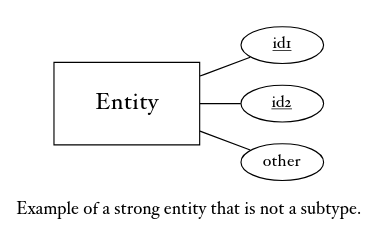
\includegraphics[width=0.5\textwidth]{ ./figures/18.png }
\begin{itemize}
    \item Make a new relation, whose name will be the same as the name of the entity
    \item The \textit{primary key} of the relation will be all of the identifier attributes, taken together
    \item All attributes of the entity become attributes of the relation.
\end{itemize}
\end{figure}
Schema of new relation from entity pictured above: \textit{\textbf{Entity}}(\underline{idr}, \underline{id2}, other)
\subsubsection{Strong Entity, Subtype}
\begin{figure}[H]
\centering
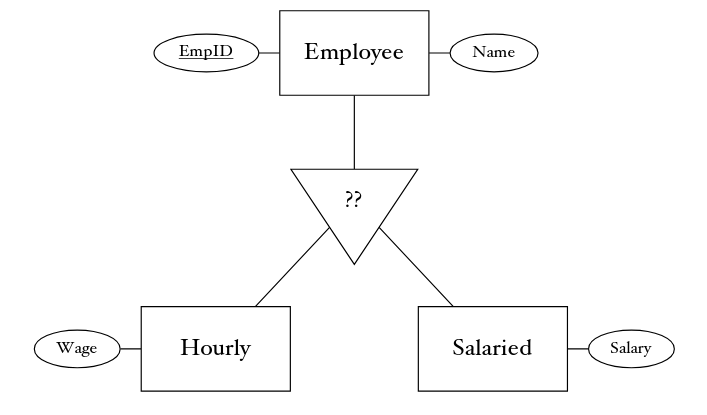
\includegraphics[width=0.5\textwidth]{ ./figures/21.png }
\end{figure}

\textit{\textbf{Employee}} is a supertype (not subtype) so it gets handled in the previous step.
\begin{itemize}
    \item \textit{\textbf{Employee}}(\underline{EmpID}, Name)
\end{itemize}
\textbf{Hourly} and \textbf{Salaried} are each strong, but they are subtypes (each is a type of \textbf{Employee}), so they are handled here.
\begin{itemize}
    \item This type of inheritance means that the subtypes \textit{are} types of the supertype, so they are identified by \textbf{Employee's} EmpID.
    \item There are \textit{two} methods for handling these subtypes.
\end{itemize}
\subsubsection*{Method 1 - Big Table}
The first method involves putting the attributes of the subtypes into the relation made for the supertype. So, the original relation:
\begin{itemize}
    \item \textit{\textbf{Employee}}(\underline{EmpID},Name)
\end{itemize}
Would become something like:
\begin{itemize}
    \item \textit{\textbf{Employee}}(\underline{EmpID}, Name, Wage, Salary)
\end{itemize}
But it would beed to be modified to indicate which subtypes a given employee belongs to. This is handled differently depending on the IS-A's configuration
\begin{itemize}
    \item For \textit{disjoint subtypes}, where an instance of the supertype can only be one of the subtypes at a time, we can add an attribute, EmpType that has a value indicating which type this employee is:
        \begin{itemize}
            \item \textit{\textbf{Employee}}(\underline{EmpID}, Name, EmpType, Wage, Salary)
        \end{itemize}
\end{itemize}
\nt{
    For \textit{generalization}, EmpType would not allow \texttt{NULL}. For \textit{specialization}, it would be allowed.
}
\begin{itemize}
    \item For \textit{overlapping subtypes}, it is possible to be more than one at a time, so we need an individual true/false answer for each type:
        \begin{itemize}
            \item \textit{\textbf{Employee}}(\underline{EmpID}, Name, IsHourly, Wage, IsSalaried, Salary)
        \end{itemize}
\end{itemize}
In this case, nothing about the schema would indicate \textit{generalization} vs. \textit{specialization.}
\newpage
\noindent Below is an example of what some instance data for the design above could look like:
    \begin{figure}[H]
    \centering
     \setlength{\tabcolsep}{20}
    \begin{tabular}{llllll}
    \toprule 
    EmpID&Name&IsHourly&Wage&IsSalaried&Salary \\
    \midrule
    1& Jim& false& NULL & true & \$56,000\\
    2&Bob&true&\$20.00&false&NULL \\
    3&Sally&false&NULL&true&\$75,000 \\
    4&Jane&false&NULL&true&\$65,800\\
    5&Arvind&true&\$5.00&true&\$60,000\\
    \bottomrule
    \end{tabular}
    \end{figure}
\noindent Note that, while it is probaly not common for someone to be both hourly and salaried, this design would support that.
\subsubsection*{Method 2}
Method 2 involves creating a new relation for the subtype entity.
\begin{itemize}
    \item The name of new relation would be the same as the name of the entity.
    \item The \textit{primary key} of the new relation would be the same as the \textit{primary key} for the supertype's relation.
    \item The \textit{primary key} is also a \textit{foreign key} to the existing table.
    \item An instance of the supertype entity will only have a tuple in the subtype relation if it is a member of that subtype, so we will not need any extra attribute like we did in method 1.
    \item The \textit{foreign key} can be used to look up any of the attributes that are being inherited from the supertype.
\end{itemize}
\bigbreak \noindent
The supertype table remains unchanged with method 2:
\begin{itemize}
    \textit{\textbf{Employee}}(\underline{EmpId}, Name)
\end{itemize}
The subtypes each get their own table.
\begin{itemize}
    \item \textit{\textbf{Hourly}}(\underline{EmpID\dag}, Wage)
    \item \textit{\textbf{Salaried}}(\underline{EmpID\dag}, Salary)
\end{itemize}
The (\dag) will be used in these slides to indicate that the attribute is part of a \textit{foreign key} (and, in this example, the whole thing).
\bigbreak \noindent
In method 2, the supertype table is not changed, so the same data we used in the previous method would look like this:
\bigbreak \noindent
\textit{\textbf{Employee}} (supertype entity)
    \begin{figure}[H]
    \centering
     \setlength{\tabcolsep}{30}
    \begin{tabular}{ll}
    \toprule 
    EmpID&Name \\
    \midrule
    1& Jim \\
    2& Bob\\
    3& Sally \\
    4& Jane \\
    5& Arvind \\
    \bottomrule
    \end{tabular}
    \end{figure}
    \newpage
    
\noindent    \textit{\textbf{Hourly}} (subtype entity)
    \begin{figure}[H]
    \centering
     \setlength{\tabcolsep}{30}
    \begin{tabular}{ll}
        \toprule
    EmpID & Wage  \\
    \midrule
    2&\$20.00 \\
    5& \$5.00 \\
    \bottomrule
    \end{tabular}
    \end{figure}
    \bigbreak \noindent
    \textit{\textbf{Salaried}} (subtype entity)
        \begin{figure}[H]
        \centering
         \setlength{\tabcolsep}{30}
        \begin{tabular}{ll}
        \toprule 
        EmpID&Salary \\
        \midrule
        1&\$56,000 \\
        3&\$75,000 \\
        4&\$65,800 \\
        5&\$60,000 \\
        \bottomrule
        \end{tabular}
        \end{figure}
        \subsubsection{Weak Entity}
        \begin{figure}[ht]
        \centering
        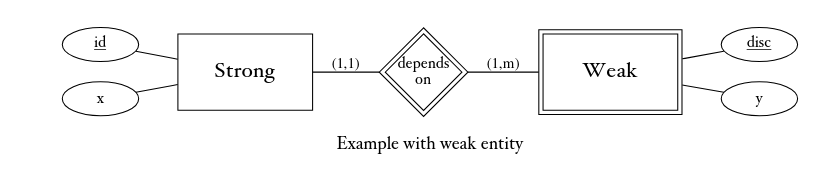
\includegraphics[width=0.8\textwidth]{ ./figures/04.png }
        \end{figure}
\noindent            The strong entity would already have a relation from section 1.1.1
\begin{itemize}
    \item \textit{\textbf{Strong}}(\underline{id}, x)
\end{itemize}
The weak entity gets its own relation. The \textit{primary key} will be the concatenation of the weak entity's \textit{discrimator} with the strong entity's \texit{identifier}. The other attributes of the entity are brought in as non-prime attributes.
\begin{itemize}
    \item \textit{\textbf{Weak}}(\underline{id\dag}, \underline{disc},y)
\end{itemize}
The \textit{identifier} portion is a \texit{foreign key} to the \textbf{Strong} relation.
\nt{
    A \textit{discriminator} looks like an \textit{identifier} (underlined attribute), but it is attached to a \textit{weak entity}.
}
\subsubsection{Entities: Functional Dependencies}
The only \textit{functional dependencies} introduced by the entites of an ER diagram are the ones introduced when the \textit{identifiers} become \textit{primary keys}. Remember that a primary key has to functioanlly determine all of the other attributes in a relation.
\subsection{Step 2: Handle Relationships}
\end{document}
